\documentclass[a4, titlepage]{article}

\usepackage[czech]{babel}
\usepackage[utf8]{inputenc}
\usepackage[T1]{fontenc}

\usepackage{graphicx}
\graphicspath{ {./img/} }

\usepackage{hyperref}
\hypersetup{
    colorlinks=true,
    linkcolor=blue,
    filecolor=magenta,      
    urlcolor=yellow,
}
\usepackage{listings}

\begin{document}

\title{Dokumentace k semestrální práci z předmětu KIV/DBM2}
%\subtitle{AlaSQL}
\author{Bc. Tomáš Vyleta}
\date{}

\maketitle

\tableofcontents
\newpage

\section*{Úvod}
Problémem či zadáním semestrální práce je nalézt a popsat knihovnu pro zpracování množiny souborů ve formátu JSON, které většinou vrací endpointy REST API. Využít ji na úrovni jednoho programu (bez nutnosti vkládání dat do jiných SŘBD pro zpracování objektových souborů). Knihovna by měla být schopna poskytovat funkce obsažené v jazyce SQL jako FROM, GROUP BY, JOIN, atd. Cíle práce jsou: 

\begin{itemize}
	\item Nalezněte existující metody dotazováním se nad množinou JSON souborů.
	\item Popište rozsah nabízených operací ve vybraném jazyce/nástroji.
	\item Analyzujte možnosti jazyka/nástroje v kontrastu s klasickou relační databází resp. SQL.
\end{itemize}


\section{Knihovna AlaSQL}
AlaSQL (čti à la SQL)je \textit{open source} SQL databáze pro JavaScript, operující na straně klienta. Implementuje mnoho funkcí ze čtvrté verze jazyka SQL (SQL:1999) a také některé funkce navíc pro snazší manipulaci s NoSQL a grafovými sítěmi. Také podporuje asynchronní volání pomocí metody promise. Knihovnu lze využít pro webové aplikace, aplikace založené na Node.js nebo v mobilních aplikacích.

Podporuje import/export formátů, jako jsou např. tabulky programu Excel (.xls), CSV - Comma-separated values (.csv), již zmiňovaný JSON - JavaScript Object Notation (.json), TAB - Tab Separated Data File (.tab) a import/export databází IndexedDB, LocalStorage a SQLite.

\begin{figure}[h]
    \centering
    
\includegraphics[width=5cm]{alasql_logo}
    \caption{Logo AlaSQL}
\end{figure}

Užitečné odkazy:
\begin{itemize}
	\item WEB: \url{http://alasql.org}
	\item Github: \url{https://github.com/agershun/alasql}
\end{itemize}

\section{Stack}
Pro práci s knihovnou jsem zvolil \textit{single page} aplikaci, kde všechny dotazy běží na klientovi s podporou JavaScriptu. Aplikace neběží na žádném serveru, tudíž nelze načítat soubory pomocí běžných metod, proto jsou všechna data uložená jako proměnné v JavaScriptu. Pokud ale pracujete s knihovnou v prostředí Node.JS, můžete soubory načítat pomocí \textit{File system} modulu nebo pokud Node.JS nevyužíváte a applikace vám běží na serveru, tak je zde možnost načítat soubory např. pomocí JQuery (asynchronně) nebo pomocí dalších externích knihoven a frameworků. Alasql dokáže načítat soubory asynchronně, ale metody kterými to jde, mají divné ukládání dat viz kapitola načítání dat.

\section{Instalace}
Knihovna je dostupná v několika JavaScriptových správcích balíčků (package management) kterými jsou npm, Bover a Meteor nebo si ji můžete přímo naklonovat/stáhnout z officiálního GitHub repozitáře. 

Pokud nechcete stahovat knihovnu na fyzické úložiště, nejjednodušší varianta je získat AlaSQL do své aplikace pomocí cloudové služby \href{https://cdnjs.com/libraries/alasql}{cdnjs.com}, která je založena na principu CDN (Content Delivery Network). Stačí tedy do našeho projektu vložit odkaz na tuto knihovnu, např. do hlavičky HTML souboru:

\begin{lstlisting}[language=HTML]
<script src="//cdn.jsdelivr.net/alasql/0.2/alasql.min.js">
</script> 
\end{lstlisting}


\section{Použití}
Po úspěšném nainstalovaní/naimportování knihovny jsme schopni ji začít používat. Nyní je několik možností jak s knihovnou pracovat. 

\subsection{Pomocí funkce}
Všechny dotazy (queries) se vkládají jako atribut metody \textit{alasql(stringWithSQL)} nebo jiné proměnné, pokud si je nazvete, třeba v Node.js. Dotazy lze vykonávat také nad jednotlivou tabulkou nějaké databáze pomocí funkce \textit{exec()} (viz dále).

\subsubsection{NodeJS}
\begin{lstlisting}
var alasql = require('alasql');
alasql('CREATE TABLE one (two INT)');
\end{lstlisting}

\subsection{Nová databáze}
Můžeme do proměnné založit novou databázi a nad vytvořenou proměnnou zavolat funkci \textit{exec()} do které vložíme dotaz jako atribut jako v předchozí sekci. Můžeme také vkládat více dotazů oddělených ;, kde poté navrácená hodnota bude jako pole výsledků.

\begin{lstlisting}
var mybase = new alasql.Database();
mybase.exec('CREATE TABLE one (two INT)');
\end{lstlisting}

Funkce \textit{alasql()} je zkrácenou verzí \textit{alasql.exec()}.

Také k ním můžete přistupovat přes globální objekt \textit{alasql}. Obecně se všechny databáze nacházejí na cestě \textit{alasql.databases.[název databáze]}.

\begin{lstlisting}
var mybase = new alasql.Database('mybase');
console.log(alasql.databases.mybase);
\end{lstlisting}

\begin{figure}[h]
    \centering
    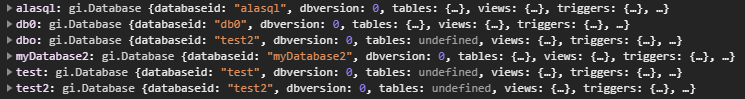
\includegraphics[width=10cm]{databases}
    \caption{Inicializované databáze v objektu \textit{alasql} (příklad)}
\end{figure}

\subsection{Nová tabulka}
Založení nové tabulky je podobné, můžeme ji vytvořit přímo v globálním objektu \textit{alasql} nebo vytvořit do nějaké databáze. Budu předpokládat, že máme databázi uloženou v proměnné \textit{var mybase}. Založení tabulky je pak následující:

\begin{lstlisting}
mybase.exec("CREATE TABLE cities (city string, population 
number)");
console.log(alasql.databases.mybase.tables.cities);
console.log(mybase.exec("SELECT * FROM cities"));
\end{lstlisting}

Jak můžete vidět, výpis celé tabulky může být uskutečněn opět pomocí cesty \textit{alasql.databases.[název databáze].tables.[název tabulky]} nebo jako SQL dotaz nad databází.

\subsubsection{Datové typy}
Datové typy, které jsou dostupné od začátku, tak se dají nalézt v \textit{alasql} objektu pod cestou \textit{alasql.fn.[název nového dat. typu] = [Datový typ]}. V základu jsou k dispozici tyto datové typy:
\begin{figure}[h]
    \centering
    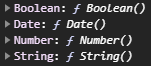
\includegraphics[width=5cm]{fn}
    \caption{Základní datové typy}
\end{figure}

Příklad přidání nového datového typu do objektu databáze:
\begin{lstlisting}
// novy datovy typ
alasql.fn.Date = Date;
    alasql('CREATE order (orderno INT, orderdate Date)');
\end{lstlisting}

\subsection{Manipulace dat v tabulce}
Jako jsme zvyklí z SQL, data jsou provádět různé úkony, jako je INSERT, UPDATE a DELETE. Syntaxe je stejná jako při založení nové tabulky. Akorát se změní dotaz. Jako příklad mohu uvést:

\begin{lstlisting}
mybase.exec("INSERT INTO cities VALUES ('Rome',2863223), 
('Paris',2249975), ('Berlin',3517424),  
('Madrid',3041579)");
\end{lstlisting}

\subsubsection*{INSERT jako JS funkce}
Knihovna umožňuje také vytvářet vlastní metody a jedna z možností je přes funkci \textit{compile()} knihovny, která umožňuje překompilovat příkazy a přidá je do cache dané databáze.

\begin{lstlisting}
var insert1 = db.compile('INSERT INTO one (?,?)');
var insert2 = db.compile('INSERT INTO one (:a,:b)');

insert1([1,2]);
insert2({a:3,b:4});
\end{lstlisting}


\subsubsection*{Přidělení dat jako JS objekt}
Určitě vás napadlo, že jako přistupujeme k databázím a tabulkám přes globální objekt, proč by nešlo přistupovat i k datům tabulky nebo je rovnou přiřadit a opravdu to jde. Obecně se všechna data tabulky nacházejí v \textit{alasql.databases.[název databáze].tables.[název tabulky].data}. Příklad objekt na přidělení dat může být následující:

\begin{lstlisting}
const ceskaMesta = [
    {name: 'Prague', population: 1324277},
    {name: 'Brno', population: 381346},
    {name: 'Ostrava', population: 287968},
    {name: 'Plzen', population: 174842}
];
alasql.databases.mybase.tables.cities.data = ceskaMesta;
\end{lstlisting}

Je zde ale riziko, přidělená data neprochází přes žádnou funkci, tudíž data vůbec nemusejí odpovídat schématu tabulky, při přidělení dat žádná vyjímka nevyhodí, ale pokud by jsme nad daty zavolali nějaký dotaz, vyskočila by podmínka nebo by data byla \textit{undefiend}. 

\subsection{Načítání souborů}
V dokumentaci je uvedené, že lze zřídit databázi z lokálního souborového systému nebo ze souboru SQLite (místo výroku FILESTORAGE -> SQLITE) a IndexedDB (místo výroku FILESTORAGE -> INDEXEDDB)
\begin{lstlisting}
alasql('ATTACH FILESTORAGE DATABASE 
test("./js/file.json")', function () {
    console.log(alasql.databases.test.data);
});
\end{lstlisting}
Vytvoří se databáze s názvem \textit{test} s daty, která jsou v atributu data v dané databázi. Tento atribut pro jinak založené databáze není běžný, jelikož atribut data neobsahují, mají je až obsaženy v tabulkách databáze. Nepřišel jsem na způsob jak nad těmito daty použít dotazy, pouze jak přes adresu proměnné vypsat všechna data nebo dotazovat se pomocí placeholderu s odkazem na data.
Je možné, že podporované databáze mají v souboru založené tabulky a Alasql je sám namapuje, pak lze nad nimi vyvolávat dotazy bez vyhození chyby.

\section{Synchronní/Asynchronní přístup}
Za normálního běhu knihovna vykonává procesy synchronně, ale jdou také volat callbacky nebo asynchronní volání pomocí metody \textit{promise()}. Pokud pracujete se soubory, načítáte je, pak knihovna funguje asynchronně a je doporučeno používat již zmíněnou metodu \textit{promise()}.

\begin{lstlisting}
// callback
alasql('SELECT * FROM cities', [],
    function (res) {
        console.log(res);
    }
);

// promise
alasql.promise('SELECT * FROM cities')
    .then(function(res){
    // zpracovani response
    }).catch(function(err){
    // zpracovani chyby
});
\end{lstlisting}

\subsection{HTML}
Knihovna dokáže číst data z HTML tabulky <table>...</table> a výsledek opět vygenerovat do HTML tabulky.
\begin{lstlisting}[language=SQL]
// cteni z tabulky
alasql('SELECT * FROM HTML("#MyTable", {headers:true})');

// zapis do tabulky
alasql('SELECT * INTO HTML("#MyTable", {headers:true}) 
FROM ?',[data]);
\end{lstlisting}


\section{SQL dotazy}
Knihovna podporuje všechny základní výroky SQL jazyka, jako jsou JOIN, GROUP, UNION, ANY, ALL, IN, podotazy a také okleštěnou správu transakcí. Dále také knihovna podporuje agregační data mining??? funkce, kterými jsou ROLLUP, CUBE a GROUPING SETS.

\subsection{Nejlépe funguje s JS}
Tato knihovna je v podstatě SQL databáze v JavaScriptu. Slouží zejména jako podpora zpracování, usnadnění délky kódu, lepší práci s daty nebo jako samostatná databáze - nejlépe však funguje \textbf{SPOLEČNĚ} s JavaScriptem. Knihovna nevrací rovnou tabulky, jak je běžné u relačních databází, ale defaultně vrací data právě jako JSON a další práce s ním je už jako práce s objektem. Sami autoři ve své dokumentaci uvádějí nějaké příklady společně s JavaScriptem a pokud příliš neznáte knihovnu nebo nevíte že nějaké funkce obsahuje, je snazší zpracovat dotaz pomocí JavaScriptu.

\begin{lstlisting}
// vypis poctu objektu ve vracenem poli
var db = new alasql.Database();
db.exec('select * from one', function(data) { // callback
   console.log(data.length);						
});

// novy datovy typ
alasql.fn.Date = Date;
    alasql('CREATE order (orderno INT, orderdate Date)');
\end{lstlisting}

\section{Datasety}
\subsection{Rohlík.cz}
K dispozici máme data z webového portálu Rohlik.cz, který se zaměřuje na obchod s potravinami. Data obsahují dva soubory ze dne 2.11.2020, jeden z pohledu obyčejného uživatele (\textit{rohlik2.json}) a druhý z pohledu prémiového uživatele (\textit{rohlik1.json}), hlavní rozdíl mezi těmito dvěma datasety je v ceně za dopravu. Nejvíce nás zajímá atribut \textit{availabilityDays}, který se sestává ze čtyř dalších objektů, popisující dnešek a další následující tři dny. V nich nalezneme atribut \textit{slots}, ve kterém jsou objekty popisující hodiny daný den. V dané hodině nás zajímá atribut \textit{timeSlotCapacityDTO}, který obsahuje konečný atribut \textit{totalFreeCapacityPercent} popisující obsazenost danou hodinu. O úroveň víš je pak atribut \textit{price} značící cenu dovozu.

\subsection{Starcraft}
Druhým datasetem jsou data ze hry Starcraft, máme k dispozici soubory dvou typů. Prvním typem (A) je popis jednotlivých \textbf{tierů}, kterých je dohromady 6, ale k dispozici máme pouze 5. a 6. Dále každý tier obsahuje pole po třech \textbf{divizích (úrovních)} kromě poslední 6. - ta obsahuje pouze jeden. Division má atributy \textit{min\_rating} a \textit{max\_rating} určující rozmezí hráčů. Každý division má pole  obsahuje pole s několika \textbf{laddery}, které již obsahují jednotlivé hráče. Tyto laddery se v průběhu času mění a maximální počet hráčů v jednom ladderu je 100. Laddery popisují soubory typu B, které jsou ve dvou různých datech. Jednotlivé laddery se dají rozeznat podle id a timestampu. V souborech je uložené pole \textit{team} které obsahuje data o jednotlivých hráčích, muhu uvést některé, které budu používat, např. \textit{last\_played\_time\_stamp} - udávající poslední aktivitu hráče v ms, \textit{member[0].legacy\_link.name} - nick hráče s rozeznávacím tagem, \textit{member[0].played\_race\_count.race} - udávající rasu, za kterou hráč hrál, atd.

\section{Důležitá je cesta, ne cíl}
V této sekci popíši všechny dotazy, které jsem pomocí Alasql řešil, jak jsem postupoval a popř. co se mi nepovedlo nebo knihovna nenabízí. 

\subsection{Rohlík.cz}
\subsubsection{Jaké je nejbližší okno s volnou kapacitou?}
Tento dotaz jsem musel řešit s pomocí JavaScriptu, jelikož struktura dat Rohlik.cz v \textit{slots} (rozvozová okénka) jsou atributy a tudíž nelze procházet tento atribut v Alasql jako pole, ale pouze přímými adresami na jednotlivé objekty, pokud chceme projít všechny rozvozová okénka, musíme použít k iteraci JavaScript. V tomto dotazu nám jde o nalezení nejbližšího volného okénka, což je nalezení takové hodnoty, kdy \textit{totalFreeCapacityPercent} je větší než 0: 
\begin{lstlisting}
(alasql('SELECT slots FROM ?'
,[rohlikPremium.data.availabilityDays]).forEach(day => {
    for (const [key, value] of Object.entries(day.slots)) {
        const freeCapasity = 
        (alasql('SELECT timeSlotCapacityDTO->totalFreeCapacityPercent 
        AS freeCapacity FROM ?',[value]));
        if (freeCapasity[0].freeCapacity > 0) {
            console.log('Prvni volne okenko dne je: '
             + value[0].since + ' do ' + value[0].till) ;
            break;
        }
    }
}));
\end{lstlisting}
Prvním dotazem vybereme pomocí Alasql atribut \textit{slots}, což je pole (dotaz je zde zbytečný, stačilo pouze přistoupit k poli pomocí JavaScriptu, ale chtěl jsem co nejvíce využívat Alasql). Procházíme každý den. Po té iterujeme každým časovým okénkem pomocí metody for pro iteraci objektů. V každém okénku si necháme pomocí dotazu napsaného v Alasql najít zanořený atribut \textit{totalFreeCapacityPercent} a pomocí podmínky zjistit, jestli je větší jak 0, pokud ne opakujeme a pokud ano, tak necháme časové okénko vypsat a danou iteraci zrušíme pomocí break a iterujeme na další den. Tím se nám vypíší všechny okénka v každém dni:
\begin{figure}[h]
    \centering
    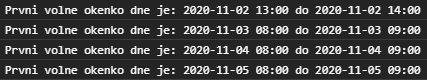
\includegraphics[width=10cm]{R1}
    \caption{Logo Výsledek dotazu Rohlik.cz - 1}
\end{figure}

\subsubsection{Kolik volných časových intervalů je k dispozici?}
Tento dotaz je podobný jako první, akorát nechceme pouze najít první volné časové okénko, ale všechny v ten daný den. Tudíž v podmínce nebudeme chtít iteraci přerušit, ale pouze aby pokračovala a pokud tam je volné okénko, tak ho přičíst k nějakému counteru a vypsat pro jednotlivý den, výsledek je: 
\begin{figure}[h]
    \centering
    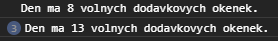
\includegraphics[width=10cm]{R2}
    \caption{Logo Výsledek dotazu Rohlik.cz - 2}
\end{figure}

\subsubsection{Jaké je nejbližší nejlevnější okno s volnou kapacitou?}
TODO

\subsection{Starcraft}
\subsubsection{Kolik hráčů je v jednotlivých divizích/úrovních?}
TODO

\subsubsection{Jsou konzistentní počty hráčů mezi JSON typ A a B?}
TODO

\subsubsection{Seřazení hráčů v rámci jednoho ladderu.}
S touto otázkou si knihovna poradí celkem snadno (bez pouřití JavaScriptu), pokud chceme seřadit hráče v jednom ladderu a známe id tohoto ladderu. S přiloženými daty si například vezmeme soubor \textit{ladders-eu-230898.json}, což je ladder s \textit{ladder\_id=230898} a pomocí JS můžeme přistupovat k jeho atributům. Všechny hráči daného ladderu jsou uložené v poli \textit{team}. Chceme zobrazit id hráče, k případnému dalšímu dotazování, jméno hráče a rating, což bude seřazená hodnota. Vytvoříme si AlaSQL dotaz:
\begin{lstlisting}
alasql('SELECT id, rating, member->(0)->character_link->battle_tag  
FROM ? ORDER BY rating DESC', [ladderJson.team])
\end{lstlisting}
Vybereme všechny zmíněné atributy. Atribut jména hráče je zanořený, proto musíme volit přístup přes další atributy nebo pole a zobrazíme ho jako battle\_tag, jinak by se celý atribut nazýval podle cesty, které k němu přistupujeme (v tomto případě by se vybraný atribut jmenoval 'member->(0)->character\_link->battle\_tag'). 
Vybraná data můžeme seřadit podle atributu \textit{rating}, pomocí výrazu ORDER BY sestupně nebo vzestupně. Jako výsledek dotazu nad ladderem s ladder\_id=230898 nám dotaz sestrojí následující výsledek:

\begin{figure}[h]
    \centering
    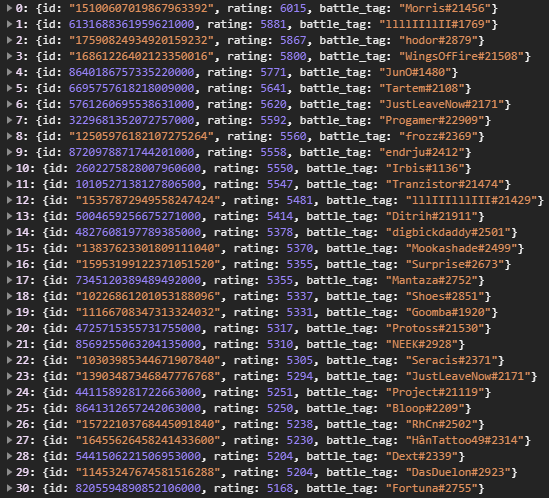
\includegraphics[width=10cm]{S3}
    \caption{Logo Výsledek dotazu Starcraft - 3}
\end{figure}

Jediné na co jsem během tohoto dotazu narazil je, že jsem chtěl, aby si uživatel volil metodu seřazení, jestli ASC nebo DESC přes placeholder pomocí ?, bohužel ale při překladu aplikace padala a vyžadovala již definovanou metodu seřazení vloženou přímo jako string v dotazu.

\subsubsection{Jací hráči vybočují z hranic divizí?}
TODO

\subsubsection{Kolik hráčů odehrálo v poslední době nějakou hru?}
K tomuto dotazu knihovně opět postačí pouze jeden dotaz, se dvěma vstupními parametry, které nahradíme místo placeholderů a to určitý ladder a konstanta času v ms proti které budeme hráče porovnávat. Alasql dotaz je:
\begin{lstlisting}
alasql.exec('SELECT COUNT(*) FROM ? WHERE 
last_played_time_stamp > ?', [ladderJson.team, timeFromInMilis])
\end{lstlisting}
Chceme zobrazit číslo, tedy počet hráčů, kolik hrálo Starcraft od časové značky. Použijeme agregační funkci COUNT buď s nějakým atributem nebo hvězdičkou, což je v tomto případě jedno. Musíme přidat také klauzuli WHERE a říci, že hledáme hráče, kteří mají \textit{last\_played\_time\_stamp} větší než naše časové razítko. Výsledkem dotazu je:

\begin{figure}[h]
    \centering
    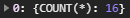
\includegraphics[width=5cm]{S5}
    \caption{Logo Výsledek dotazu Starcraft - 5}
\end{figure} 

\subsubsection{Jací hráči jsou v jednom ladderu vícekrát a za jaké rasy?}
Tento dotaz jsem se snažil vyřešit pouze s pomocí Alasql, ale k výsledku jsem se dobral pouze s pomocí JavaScriptu. Vstupním parametrem je jeden ladder.
\begin{lstlisting}
result = '';
temp = alasql('SELECT member->(0)->
character_link->battle_tag as name, member->(0)->
played_race_count->(0)->race as race FROM ?', 
[ladderJson.team]);
    alasql('SELECT name FROM ? GROUP BY name 
    HAVING COUNT(*) > 1 ORDER BY name', 
    [temp]).forEach(dupPlayer => {
        result += dupPlayer.name + ': '
        temp.forEach(player => {
            if (dupPlayer.name === player.name) {
                result += player.race + ', ';
            }
        });
        result += '\n';
    });
\end{lstlisting}
Nejdříve inicializuji prázdný string, který mi bude pomáhat s vypsáním výsledků dotazů. Nejdříve si do proměnné temp zobrazím \textit{battle\_tag} hráčů jako \textit{name} a rasu jako \textit{race} za kterou hráči hráli. V dalším dotazu zobrazím \textit{name} hráče, který se vyskytl v daném ladderu vícekrát. Po té si pomocí JavaScriptu pro každého hráče nechám vypsat jméno a rasy, za které hrál. Výsledek nad ladderem s ladder\_id=230882 vypadá takto:
\begin{figure}[h]
    \centering
    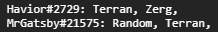
\includegraphics[width=5cm]{S6}
    \caption{Logo Výsledek dotazu Starcraft - 6}
\end{figure} 

\subsubsection{Jací hráči přibyli/ubyli v daných ladderech?}
V tomto dotazu chceme porovnat dvě instance stejného ladderu v jiných časových obdobích, tudíž vstupem budou dva zmíněné parametry. Tímto dotazem si Alasql poradí pomocí dvou dotazů nebo jedním zanořeným: 
\begin{lstlisting}
union =  (alasql('SELECT member->(0)->character_link->
battle_tag as name FROM ? UNION ALL SELECT member->(0)->
character_link->battle_tag as name FROM ?', 
[ladderJson1.team, ladderJson2.team]));

alasql('SELECT name FROM ? GROUP BY name 
HAVING COUNT(*)=1',[union])
\end{lstlisting}
Prvním krokem se sestavení UNION výroku, který vezme z obou instancí battle\_tag hráčů jako \textit{name} a vytvoří z nich pouze jednu tabulku. Nad touto tabulkou zobrazíme pouze ty hráče, kteří se v obou instancích nacházejí pouze jednou. Nevíme ale, jestli daní hráči přibili nebo ubyli. Výsledek dotazů mezi ladderem s ladder\_id=230882 je:

\begin{figure}[h]
    \centering
    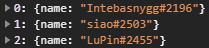
\includegraphics[width=5cm]{S7}
    \caption{Logo Výsledek dotazu Starcraft - 7}
\end{figure} 

\subsubsection{Kolik zástupců mají týmy v jednotlivých úrovních?}
TODO

\subsection{Objevené zajímavé funkce}
\subsubsection*{Placeholder}
Otazník v dotazech je tzv. placeholder. Všechny dotazy, které jsou volány přes Alasql mohou mít v dotazu otazník, který je pak nahrazen hodnotou v poli za výrazem, které obsahuje odkazy na zdroje.

\begin{lstlisting}
alasql('SELECT a->b FROM ?',[data]);
\end{lstlisting}

\subsubsection*{Vlastní funkce}
AlaSQL je rozšířitelná a umožňuje nám vytvářet vlastní funkce s použitím JavaScriptu, které pak můžeme zavolat přímo v SQL dotazu.

\begin{lstlisting}
alasql.aggr.CONCAT = function(v,s) {
    return (s||[]).concat(v);
};

alasql.aggr.LENGTH = function(array) {
	return array.length;
}
\end{lstlisting}

\subsubsection*{Abstract szntax tree}
Umožňuje převádět jazyk SQL na AST (Abstract Syntax Tree), který můžeme programově interpretovat do našeho datového modelu.

\begin{lstlisting}
var ast = alasql.parse("SELECT * FROM one");
console.log(ast.toString()); // Vypise puvodni SQL dotaz
\end{lstlisting}
Tato funkce se může použít různě, například pro rychlejší sestavování větších dotazů. Pro představu uvedu strukturu rozloženého objektu:
\begin{figure}[h]
    \centering
    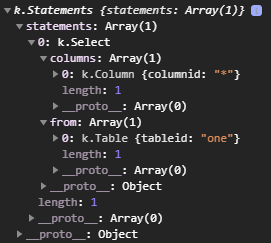
\includegraphics[width=5cm]{astObj}
    \caption{Struktura AST stromu v JavaScriptu}
\end{figure} 

\subsubsection*{pretty(sql)}
Interně, pokud se ve svých dotazech vyznáme, je tato funkce asi zbytečná, ale je dobrá ji mít při vypisování, speciálně dlouhých, dotazů do konzole nebo kamkoliv jinam. Funkce totiž zkrášlí náš stringový dotaz.

\subsubsection*{}
Místo funkcí \textit{alasql()} nebo \textit{exec()} můžete využít také jednu z následujících funkcí:

\begin{lstlisting}
alasql.value(sql, params, callback)
alasql.log(sql, params)
\end{lstlisting}

První funkce \textit{value()} vykoná dotaz, ale místo objektu nebo více hodnot vrátí pouze jednu. Druhá funkce \textit{log()} opět vykoná dotaz a rovnou výsledek vypíše do konzole nebo přímo do HTML elementu. Což se velice hodí při debugování.


\section{Chyby}
TODO
nelze prochazet promenne
nefunkci metody - napr. arrayOfArray

\section{Popis přiložených souborů}
K této dokumentaci také přikládám soubory s příklady a s řešením popsaných otázek.
TODO - popis souborů + struktura

\section{Porovnání s SQL}
Knihovna je primárně navržena aby se s ní co nejvíce pracovalo jako s SQL. Obsahuje všechny základní výroky (SELECT, DISTINC, FIRST, FROM, WHERE, ORDER BY, atd.) agregační funkce (SUM(), AVG(), GROUP BY, atd.), stringové, numerické, logické a datové funkce (ABS(), UPPER(), YEAR(), ...), JOIN operace (INNER JOIN, LEFT JOIN, OUTER JOIN, ...) a řízení transakcí příkazy (BEGIN, COMMIT a ROLLBACK). 
TODO - SQL99 standart
Pokud si vytvoříte databázi pomocí Alasql, chová se stejně jako SQL databáze, akorát ukládání dat je jiné. Data jsou uložené v JavaScriptovém objektu a máme k nim přístup i bez dotazovacího jazyka přes objektovou cestu. Data je možné ukládat i do Localstorage nebo jiné podporované databáze.

\section{Na závěr}
Celkově se mi s knihovnou dělalo relativně dobře, ALE... pouze při práci společně s JavaScriptem. Dokumentace knihovny pokrývá základy a místy je vidět, že autoři mají připravené odkazy a stránky pro její rozšíření, bohužel je v ní takový celkem zmatek, některé věci jsou na více místech a většina z "live example" nefungují. Odkaz na knihovnu z wiki je ve verzi 0.3.9, což je starší verze, přitom píší, že verze v npm je verzi 0.6.4. Jediné relevantní stránky jsou ty na GitHubu, ostatní stránky v silné většině kopírují obsah a nelze načíst další relevantní zdroj. Bohužel, což mě hodně zklamalo a trošku odradilo jsou funkce, které uvádějí se zajímavými, ne-li potřebnými funkcemi a bohužel, když si je naimplementujete do svého kódu, tak vám to většinou vyhodí exception, že požadovaná funkce zavolaná nad objektem \textit{alasql} není funkcí a nefunguje. 

Na druhou stranu, knihovna nabízí opravdu mnoho zajímavých funkcí a pomocí JavaScriptu jde udělat prakticky cokoliv. Je zde vždy několik cest, jak s knihovnou pracovat, to znamená, že je možné různé problémy řešit různými cestami. Knihovna je velmi populární, podle statistik si ji stáhne cca 13 000 lidí týdně. Leč na knihovně se stále pracuje (soudě podle commitů) a věřím, že autoři opraví stávající problémy a přidají ještě další funkce. Knihovna je opensource, takže kdyby jste potřebovali nějaký projekt na ní založit, můžete. Také pokud vám tam něco chybí, není těžké si udělat vlastní funkci, která toto vykoná. Knihovna se z velké čísti používá jako normální SQL dotazy a uživatel JavaScriptu s ní nebude mít také problémy.


\begin{thebibliography}{9}
\bibitem{notsoshort}
\textit{Github - AlaSQL} [online]. [cit. 2020-11-16]. Dostupné z: 
\url{https://github.com/agershun/alasql}

\bibitem{notsoshort}
\textit{Github - AlaSQL/Wiki} [online]. [cit. 2020-11-16]. Dostupné z: 
\url{https://github.com/agershun/alasql/wiki}

\bibitem{notsoshort}
\textit{W3C - SQL} [online]. [cit. 2020-11-16]. Dostupné z: 
\url{https://www.w3schools.com/sql/default.asp}

\bibitem{notsoshort}
\textit{cdnjs - alasql} [online]. [cit. 2020-11-16]. Dostupné z: 
\url{https://cdnjs.com/libraries/alasql}

\bibitem{notsoshort}
\textit{DZone - alasql-in-action-the-javascript-sql-database} [online]. [cit. 2020-11-16]. Dostupné z: 
\url{https://dzone.com/articles/alasql-in-action-the-javascript-sql-database}

\bibitem{notsoshort}
\textit{DEV - alasql-a-real-database-for-web-browsers-and-nodejs} [online]. [cit. 2020-11-16]. Dostupné z: 
\url{https://dev.to/jorge_rockr/alasql-a-real-database-for-web-browsers-and-nodejs-24gj}

\end{thebibliography}

\newpage
\listoffigures

\end{document}